\section{Finite Automata (FA)}
A finite automaton is the following three things:
\begin{enumerate}
    \item A finite set of states, one of which is designated as the initial state, called the \textbf{start state}, and some (maybe none) of which are designated the \textbf{final states} (or \textbf{accepting states})
    \item An \textbf{alphabet} \(\Sigma\) of input letters
    \item A finite set of \textbf{transitions} that tell for each state and for each letter of input alphabet which state to go to next:
    \begin{figure}[h!]
        \centering
        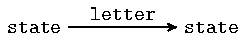
\includegraphics[]{lectures/figures/basic_fa.pdf}
    \end{figure}
\end{enumerate}
The language is \textbf{defined} or \textbf{accepted} by a finite automaton is the set of words that end in a final state.
If \(w\) is in the language defined by a finite automaton, then we also say that the finite automaton \textbf{accepts} \(w\).

Finite automaton work by being presented with an input string of letters that it reads letter by letter starting from the leftmost side.
Beginning at the start state, the letters determine a sequence of states.
The sequence ends when the last input letter has been read.
The set of all strings that end in a final state is called the language defined by the finite automaton.
The set of strings which do not end in a final state, we call not accepted or rejected by the finite automaton.

\subsection{Transition Diagram}
\begin{figure}[h!]
    \centering
    \begin{subfigure}[m]{0.2\textwidth}
        \centering
        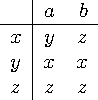
\includegraphics[width=\textwidth]{lectures/figures/transition_table.pdf}
    \end{subfigure}
    \begin{subfigure}[m]{0.5\textwidth}
        \centering
        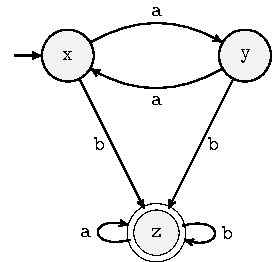
\includegraphics[width=\textwidth]{lectures/figures/transition_diagram.pdf}
    \end{subfigure}
\end{figure}
The regular expression of this FA is \(a^*b(a+b)^*\).

\subsection{Studying Automata}
\begin{enumerate}
    \item Starting with a finite automaton (FA), analyze it to determine the language it accepts.
    \item Starting from a language, build an FA.
\end{enumerate}
Example of the second method: The language of all words with an even number of letters over the alphabet \(\{a,b\}\):
\begin{itemize}
    \item Two states: 1 - even number, 2 - odd number.
    \item Start state: 1
    \item Final state: 1
    \item Transitions: \ 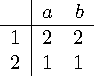
\includegraphics[width=0.2\linewidth]{lectures/figures/5-2transitions.pdf}
\end{itemize}
\begin{figure}[h!]
    \centering
    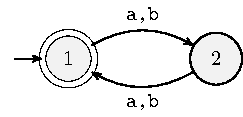
\includegraphics[width=0.4\linewidth]{lectures/figures/5-2fa.pdf}
\end{figure}

\subsection{From Languages to Finite Automata}
There is not necessarily a unique FA that accepts a given language.
Every language that can be accepted by an FA can be defined by a regular expression and, conversely, every language that can be defined by a regular expression can be accepted by some FA.
However, there are languages that are neither definable by regular expression nor accepted by an FA.
\newpage
\subsection{From Finite Automata to Languages}
Characterize states by the purposes they serve.\\
\begin{figure}[h!]
    \centering
    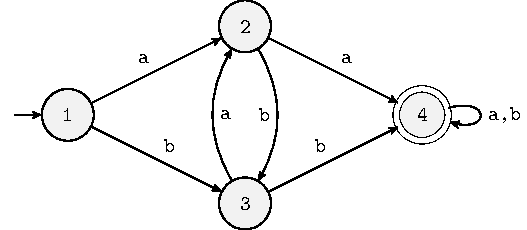
\includegraphics[width=0.6\linewidth]{lectures/figures/5-4fa.pdf}
    \caption{Finite Automata accepting the language \((a+b)^*(aa+bb)(a+b)^*\)}
\end{figure}
There are two \textquote{direct} paths to get from state 1 to state 4, either the path $1 \rightarrow 2 \rightarrow 4$ or from $1 \rightarrow 3 \rightarrow 4$. The loop between states 2 and 3 signify that there could be any number of letters at the start, this is the first \((a+b)^*\). Only when the pattern \(aa\) or \(bb\) appears we can continue to state 4, \((aa+bb)\), once in state 4, any number of letters can be accepted this is the second \((a+b)^*\). 